\documentclass[10pt,a4paper]{article}
\usepackage[a4paper,top=1.6cm,bottom=1.6cm,left=1.8cm,right=1.8cm]{geometry}
\usepackage[T1]{fontenc}
\usepackage{mathptmx}
\usepackage{graphicx,booktabs,xcolor,enumitem,amsmath,tikz,subcaption}
\usepackage[font=small,labelfont=bf,skip=3pt]{caption}
\usepackage[colorlinks=true,linkcolor=navy,urlcolor=navy,citecolor=navy]{hyperref}
\usetikzlibrary{positioning,arrows.meta,fit,backgrounds}
\definecolor{navy}{HTML}{0B3A63}
\setlength{\parindent}{0pt}\setlength{\parskip}{3pt}
\setlist{nosep,leftmargin=12pt}
\setlength{\textfloatsep}{6pt}\setlength{\floatsep}{5pt}\setlength{\intextsep}{5pt}
\newcommand{\question}[2]{\par\vspace{6pt}{\color{navy}\large\textbf{(10\%) Question #1:} #2}\par\vspace{2pt}}
\newcommand{\sub}[1]{\par\vspace{2pt}\textbf{\color{navy}#1}\quad}
\pagestyle{plain}

\begin{document}
\begin{flushright}\textit{Big Data Analytics Techniques and Applications, Fall 2026}\end{flushright}
\vspace{-8pt}
\begin{center}
{\color{navy}\Large\textbf{Assignment 3 Report:}}\\[2pt]
{\color{navy}\Large Explainable Model for Wine Quality Inference}\\[4pt]
Malo Joannon \quad$\cdot$\quad Student ID: 315551818\\[1pt] Code: \url{https://github.com/malocs15/malocs15-BigData2026-Assignment3}
\end{center}
\vspace{-6pt}\noindent\rule{\textwidth}{0.4pt}

%==========================================================================
\question{1}{Preliminary Analysis.}

\sub{Data and metric.} The training set has 15{,}000 synthetic wines (11 physicochemical features, no missing values, no duplicates); the test set has 10{,}000. Quality takes only the values 3--8 and is strongly imbalanced: 5 (42.0\%), 6 (40.4\%), 7 (12.6\%), 4 (3.1\%), 8 (1.4\%), 3 (0.6\%). Train and test feature distributions match closely (largest two-sample Kolmogorov--Smirnov statistic 0.017, for chlorides), so no covariate-shift correction was needed. The metric is the quadratic weighted kappa (QWK); I checked that \texttt{sklearn}'s \texttt{cohen\_kappa\_score(weights="quadratic")} gives exactly the value of the formula on the Kaggle Evaluation page on our predictions. QWK compares the predicted class \emph{distribution} with the true one through the expected matrix $E$, so how a continuous score is cut into classes matters as much as the score itself.

\sub{Feature analysis.} Only \textbf{alcohol} has a substantial relation with quality (Pearson 0.401, Spearman 0.391, mutual information 0.127 nats). Every other feature has $|\rho|\le0.10$ (total SO$_2$: $-0.104$) and mutual information $\le0.009$ (Fig.~\ref{fig:q1}). Two observations shaped the design: (i) the relation with alcohol is not monotone (mean alcohol is 10.33 for quality 3 but 9.81 for quality 5, then 11.14 for quality 7), which favours non-linear shape functions over a single linear term; (ii) volatile acidity, a known quality driver in the original red-wine data \cite{cortez}, has zero correlation here, so the synthetic generator appears to have weakened several chemical relations. Six domain features (total acidity, bound SO$_2$, free/total SO$_2$ ratio, alcohol$\times$sulphates, alcohol/density, volatile/fixed acidity) did not help LightGBM (CV QWK 0.4213 vs.\ 0.4220 with raw features), so the final models use the 11 raw features.

\begin{figure}[h]\centering
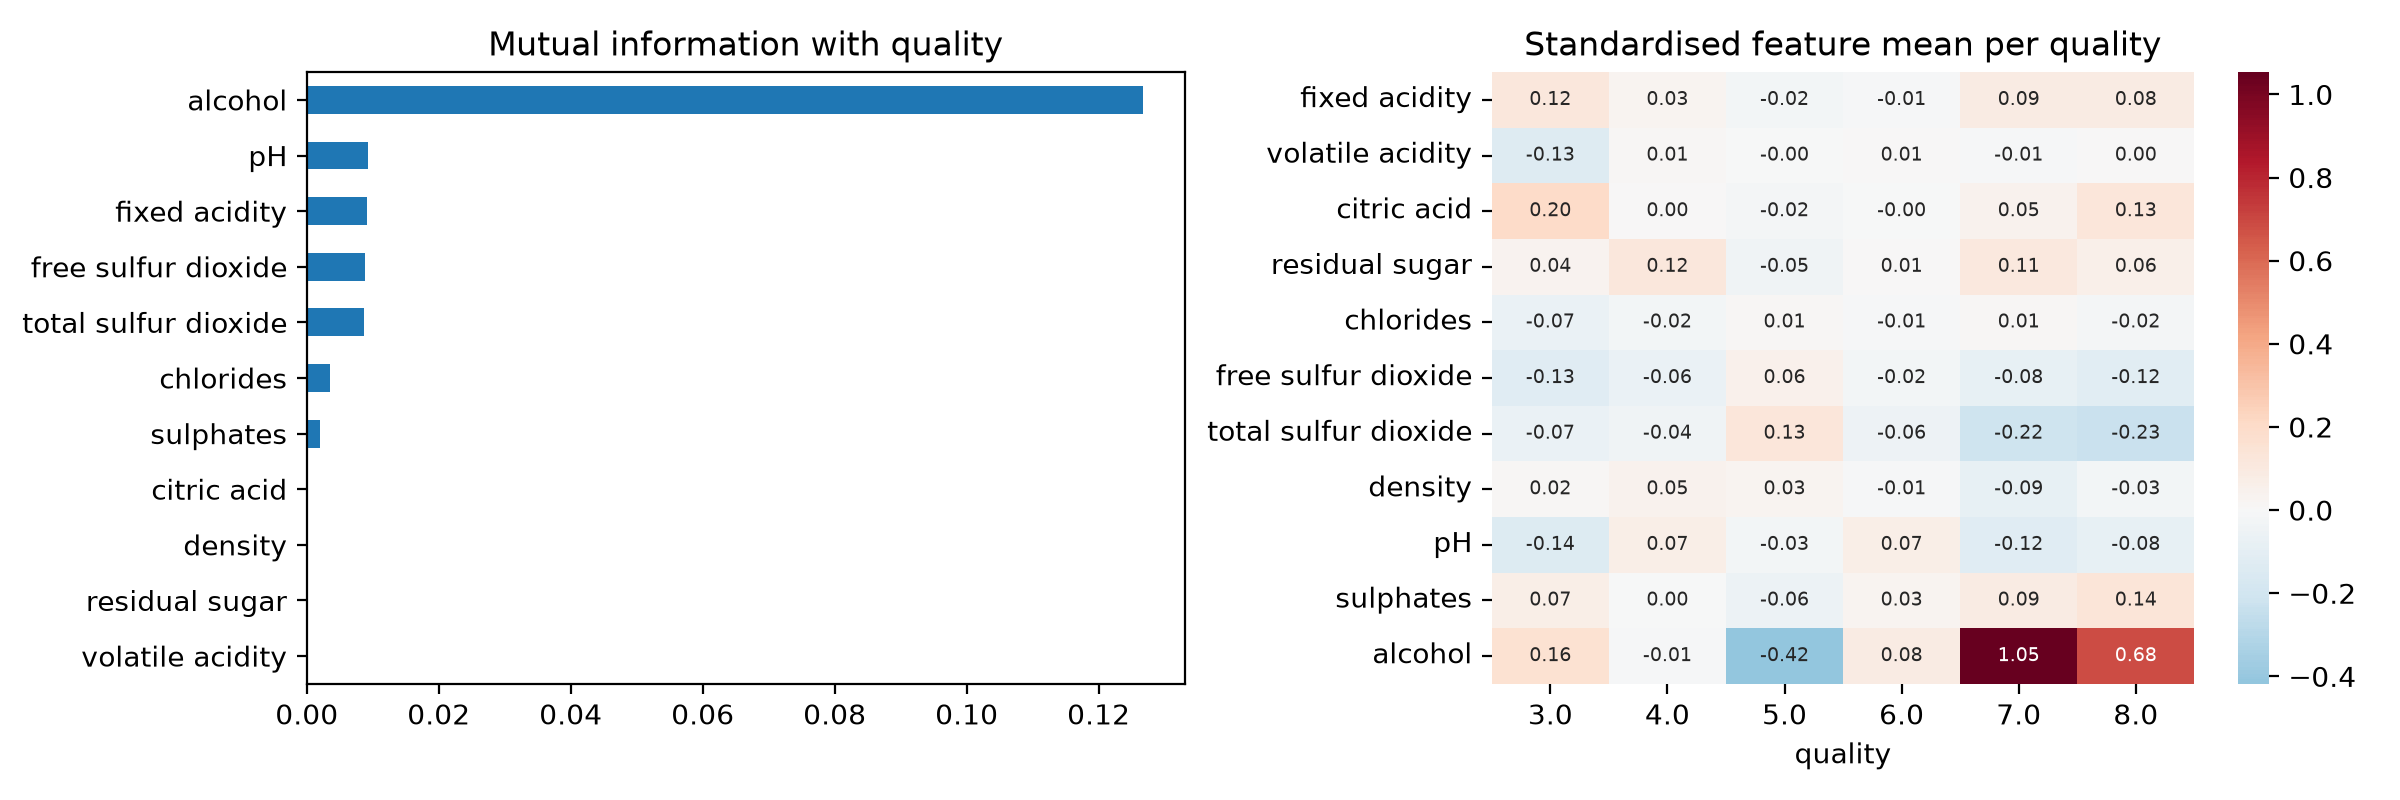
\includegraphics[width=0.86\textwidth]{../figures/q1_mi_heatmap.png}
\caption{Left: mutual information between each feature and quality. Right: standardised feature mean per quality level (red = above the overall mean).}\label{fig:q1}
\end{figure}

\sub{Baselines.} All numbers are 5-fold stratified cross-validation (CV) QWK on the training set; I used CV rather than the public leaderboard, which covers only $\approx$2{,}000 test rows (see Q3). Directly classifying the six labels gives low QWK (logistic regression 0.350, LightGBM classifier 0.346), because they almost never predict the rare classes 3, 4 and 8 and under-predict 7 (logistic regression predicts class 7 for 873 wines vs.\ 1{,}884 true). Treating quality as a continuous target and rounding is worse (Ridge 0.282), but \emph{optimising the cut points} of the regression output lifts Ridge to 0.407 and LightGBM to 0.416. Other model families did not beat regularised LightGBM (same folds, Nelder--Mead thresholds): XGBoost 0.416, LightGBM ordinal ($\sum_k P(y>k)$) 0.416, CatBoost 0.401--0.405, kNN 0.388, SVR 0.382, MLP 0.380. Conclusions: (1) treat the task as ordinal regression plus learned thresholds; (2) the signal is low and concentrated in a few features, so a sparse, interpretable model should not lose much accuracy.

%==========================================================================
\question{2}{Model Design.}

\begin{figure}[h]\centering
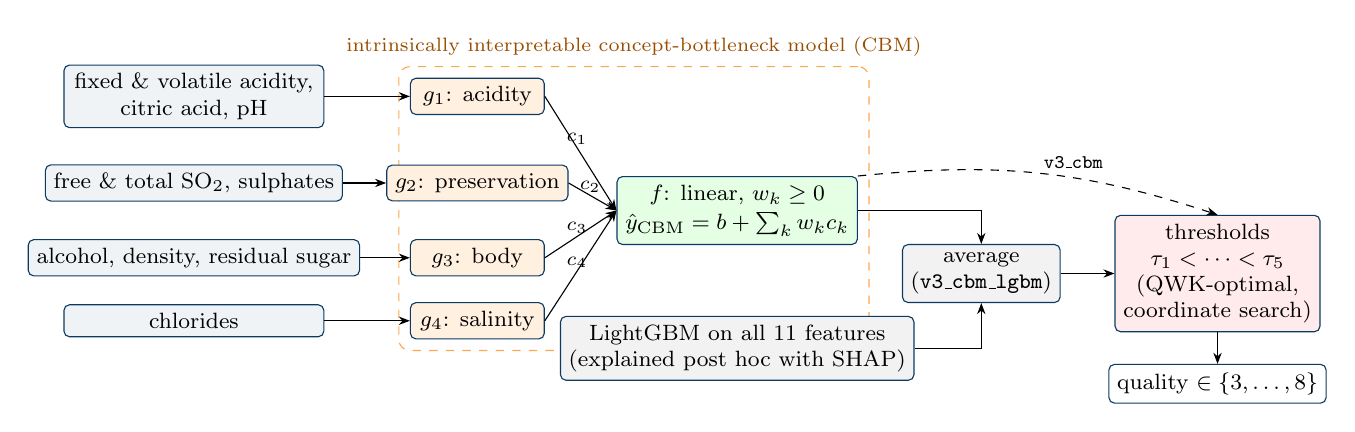
\begin{tikzpicture}[font=\footnotesize,>={Stealth[length=4pt]},
  box/.style={draw=navy,rounded corners=2pt,align=center,inner sep=3pt,fill=white},
  feat/.style={box,fill=navy!6,minimum width=3.3cm},
  cpt/.style={box,fill=orange!12,minimum width=1.7cm},
  lin/.style={box,fill=green!10}]
\node[feat] (f1) at (0,1.65) {fixed \& volatile acidity,\\ citric acid, pH};
\node[feat] (f2) at (0,0.55) {free \& total SO$_2$, sulphates};
\node[feat] (f3) at (0,-0.4) {alcohol, density, residual sugar};
\node[feat] (f4) at (0,-1.2) {chlorides};
\node[cpt] (c1) at (3.6,1.65) {$g_1$: acidity};
\node[cpt] (c2) at (3.6,0.55) {$g_2$: preservation};
\node[cpt] (c3) at (3.6,-0.4) {$g_3$: body};
\node[cpt] (c4) at (3.6,-1.2) {$g_4$: salinity};
\foreach \i in {1,2,3,4} \draw[->] (f\i) -- (c\i);
\node[lin] (f) at (6.9,0.2) {$f$: linear, $w_k\ge0$\\[1pt]$\hat y_{\mathrm{CBM}}=b+\sum_k w_k c_k$};
\foreach \i in {1,2,3,4} \draw[->] (c\i.east) -- node[above,pos=0.45,inner sep=1pt]{\scriptsize$c_{\i}$} (f.west);
\node[box,fill=gray!10] (lgb) at (6.9,-1.55) {LightGBM on all 11 features\\(explained post hoc with SHAP)};
\node[box,fill=gray!10] (avg) at (10.0,-0.6) {average\\(\texttt{v3\_cbm\_lgbm})};
\draw[->] (f.east) -| (avg.north);
\draw[->] (lgb.east) -| (avg.south);
\node[box,fill=red!8] (thr) at (13.0,-0.6) {thresholds\\$\tau_1<\dots<\tau_5$\\(QWK-optimal,\\coordinate search)};
\draw[->] (avg) -- (thr);
\draw[->,dashed] (f.north east) to[bend left=12] node[above,pos=0.6]{\scriptsize\texttt{v3\_cbm}} (thr.north);
\node[box] (out) at (13.0,-2.0) {quality $\in\{3,\dots,8\}$};
\draw[->] (thr) -- (out);
\begin{scope}[on background layer]
\node[draw=orange!70,dashed,rounded corners,fit=(c1)(c4)(f),inner sep=4pt,label={[font=\scriptsize,text=orange!60!black]above:intrinsically interpretable concept-bottleneck model (CBM)}] {};
\end{scope}
\end{tikzpicture}
\caption{Framework. Each concept model $g_k$ is a shallow LightGBM that sees only the features of its concept. The linear head $f$ is trained on out-of-fold concept scores. \texttt{v3\_cbm} thresholds the CBM output directly; \texttt{v3\_cbm\_lgbm} first averages it with a regularised LightGBM.}\label{fig:framework}
\end{figure}

\sub{Concept-bottleneck model (CBM).} Following the concept-based view of intrinsic interpretability in Lecture~6 \cite{koh}, the model is forced through a small set of human-readable wine concepts: $x\rightarrow c\rightarrow\hat y$. Since there are no concept annotations, each concept is defined by a group of features rather than by labels: acidity, preservation (sulphites), body (alcohol, density, sugar) and salinity. Each $g_k$ is a shallow LightGBM (7 leaves, 400 trees, learning rate 0.02, $\ge$80 samples per leaf, $L_2{=}5$) trained to predict quality from its group only, so $c_k$ is ``the quality suggested by this concept alone''. As in the \emph{sequential bottleneck} of Lecture~6, $g$ is trained first; the head $f$ is a linear regression fitted on 5-fold out-of-fold concept scores, so it does not learn from over-fitted $c_k$. The weights are constrained to $w_k\ge0$, so every weight reads as ``how much the model trusts this concept'' and a weight can never flip a concept's meaning. The prediction decomposes exactly as $\hat y=b+\sum_k w_k c_k(x)$.

\sub{From score to class.} QWK rewards matching the label distribution, so I learn five cut points $\tau_1<\dots<\tau_5$ that maximise QWK on the out-of-fold predictions. Nelder--Mead alone often stopped in a local optimum, so I refine its result with a coordinate search (each $\tau_k$ is grid-searched between its neighbours, 3 sweeps). Thresholds are averaged over the 3 CV seeds (42, 7, 2026). Test predictions are averaged over 15 models (3 seeds $\times$ 5 folds).

\sub{Balancing explainability and performance.} Each part keeps the model explainable while staying accurate: (1) the bottleneck has only 4 inputs, and $f$ is linear and non-negative; (2) inside a concept, $g_k$ can still learn non-linear shapes (e.g.\ the stepwise alcohol effect); (3) interactions are allowed only \emph{inside} a concept, which keeps the explanation additive at the concept level. The cost is small: the CBM alone reaches CV QWK 0.4210 versus 0.4216 for an unconstrained LightGBM, which supports Rudin's argument that interpretability need not cost accuracy \cite{rudin}. For the leaderboard I also submit the average of CBM and LightGBM (CV 0.4228). This adds a black-box part, so its explanation relies on post-hoc SHAP \cite{shap}; Q4 shows that SHAP and the CBM agree.

%==========================================================================
\question{3}{Ablation Study.}

\textbf{Final public leaderboard scores:} \texttt{v3\_cbm} \textbf{0.4427} (intrinsic CBM) and \texttt{v3\_cbm\_lgbm} \textbf{0.4423} (CBM + LightGBM). Both are above Baseline~3 (0.4364).

\begin{table}[h]\centering\small
\begin{tabular}{@{}llccc@{}}\toprule
 & Model / component & Thresholds & CV QWK (mean $\pm$ std, 3 seeds) & Public LB \\\midrule
1 & Ridge (linear baseline) & rounding & 0.2823 $\pm$ 0.0008 & -- \\
2 & Ridge & Nelder--Mead & 0.4065 $\pm$ 0.0007 & -- \\
3 & LightGBM (regularised) & rounding & 0.3329 $\pm$ 0.0011 & -- \\
4 & LightGBM & Nelder--Mead & 0.4164 $\pm$ 0.0007 & -- \\
5 & LightGBM & NM + coordinate & 0.4216 $\pm$ 0.0006 & -- \\
6 & EBM \cite{ebm} (intrinsic GAM) & NM + coordinate & 0.4184 $\pm$ 0.0017 & -- \\\midrule
7 & CBM & rounding & 0.3278 $\pm$ 0.0007 & -- \\
8 & CBM (\texttt{v2\_cbm}) & Nelder--Mead & 0.4165 $\pm$ 0.0005 & 0.4329 \\
9 & \textbf{CBM} (\texttt{v3\_cbm}) & NM + coordinate & 0.4210 $\pm$ 0.0007 & \textbf{0.4427} \\
10 & CBM + EBM + LightGBM (\texttt{v2\_blend}) & Nelder--Mead & 0.4178 $\pm$ 0.0006 & 0.4387 \\
11 & \textbf{CBM + LightGBM} (\texttt{v3\_cbm\_lgbm}) & NM + coordinate & \textbf{0.4228 $\pm$ 0.0005} & 0.4423 \\\bottomrule
\end{tabular}
\caption{Ablation. CV thresholds are fitted per seed on out-of-fold predictions. For the submitted files, thresholds averaged over seeds give CV 0.4198 (\texttt{v3\_cbm}) and 0.4215 (\texttt{v3\_cbm\_lgbm}). An earlier Ridge + LightGBM submission scored 0.4428 on the public LB with CV only 0.4138.}\label{tab:abl}
\end{table}

\sub{Effect of each component.}
\begin{itemize}
\item \textbf{Threshold learning is the largest gain} (+0.09 for every model: rows 1$\to$2, 3$\to$4, 7$\to$8). With rounding, 98\% of the predictions are 5 or 6.
\item \textbf{Coordinate refinement} adds +0.004--0.005 CV (rows 4$\to$5, 8$\to$9). It holds on unseen data: when thresholds are fitted on 4/5 of the out-of-fold predictions and scored on the remaining 1/5, CBM goes from 0.4149 to 0.4191 and CBM + LightGBM from 0.4168 to 0.4209. The refined cut points predict class 8 for 3--4\% of test wines (the last CBM cut point moves from 7.59 to 6.36), whereas the Nelder--Mead cut points never predicted it. On the public LB, the same model gains +0.0098 (\texttt{v2\_cbm}$\to$\texttt{v3\_cbm}).
\item \textbf{The concept bottleneck costs almost nothing}: CBM 0.4210 vs.\ LightGBM 0.4216, and it beats the EBM (0.4184) and Ridge (0.4087) under the same thresholds.
\item \textbf{Blending} CBM with LightGBM adds only +0.0012 CV, a sign that both capture the same signal.
\end{itemize}

\begin{table}[h]\centering\small
\begin{tabular}{@{}lccccc@{}}\toprule
CBM concepts & all four & $-$ acidity & $-$ salinity & $-$ preservation & $-$ body \\\midrule
CV QWK (seed 42) & 0.4208 & 0.4210 & 0.4206 & 0.4196 & 0.1414 \\\bottomrule
\end{tabular}
\caption{Concept ablation: one concept removed and the CBM retrained.}\label{tab:cpt}
\end{table}
\vspace{-4pt}
\textbf{Concept ablation} (Table~\ref{tab:cpt}). Removing \emph{body} destroys the model (0.14). Removing \emph{preservation} costs 0.0012. Acidity and salinity carry no measurable signal, which matches the weights learned in Q4.

\sub{Additional analysis: how reliable is the public leaderboard?} I re-scored our out-of-fold predictions on 500 random 2{,}000-row subsets, the size of the public split. One model's score varies with a standard deviation of 0.019 across subsets. Among 11 of our models with almost equal true QWK (0.419--0.422), the best and worst on the same subset differ by 0.0105 on average, and keeping the best of the 11 adds +0.005 on its own. Gaps of about 0.01 on the public LB therefore say little about the private split. For this reason I chose the models by CV, which uses 15{,}000 rows and 3 seeds and varies by less than 0.001.

%==========================================================================
\question{4}{Model Explainability.}

\sub{Type of explanation.} The CBM is \textbf{intrinsically interpretable}: its output is $\hat y=b+\sum_k w_k c_k(x)$, so the explanation \emph{is} the model's computation, without approximation. It explains at three levels: (a) the global weights $w_k$; (b) the shape of each concept score $c_k$ as a function of its features (partial dependence); (c) a per-wine decomposition $w_k\,(c_k(x)-\bar c_k)$, which shows how far each concept pushes this wine from the average wine. For the CBM + LightGBM submission, the LightGBM part is explained \textbf{post hoc} with TreeSHAP \cite{shap}.

\begin{figure}[h]\centering
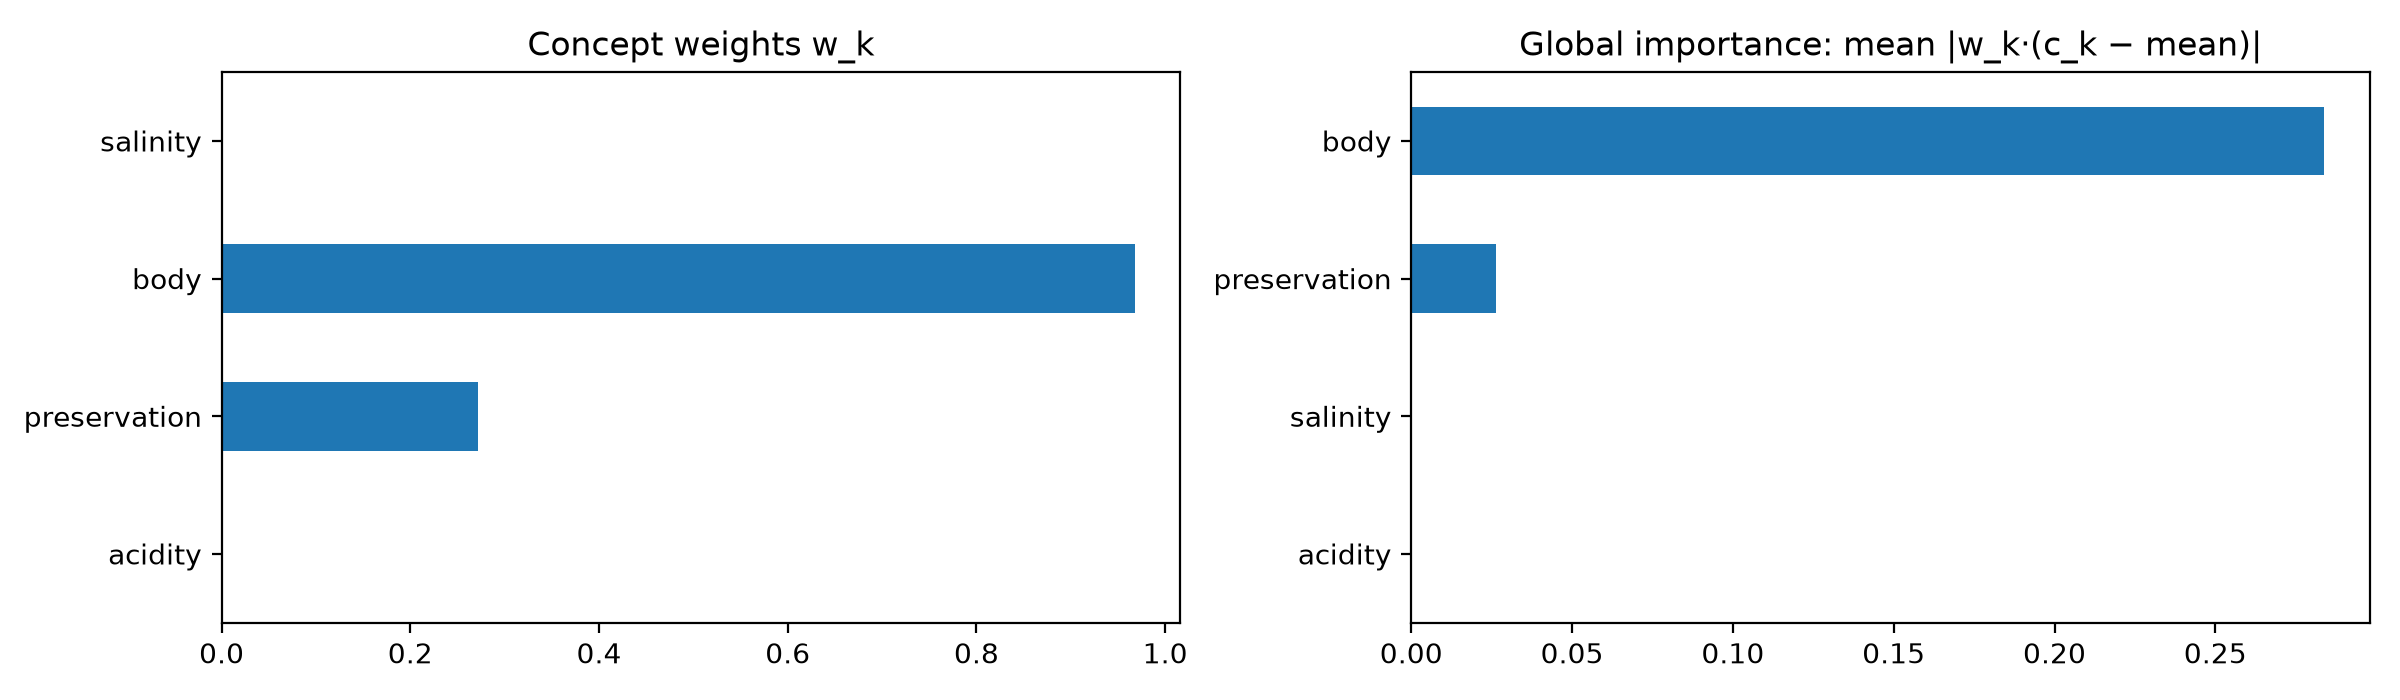
\includegraphics[width=0.83\textwidth]{../figures/q4_cbm_global.png}\\[-1pt]
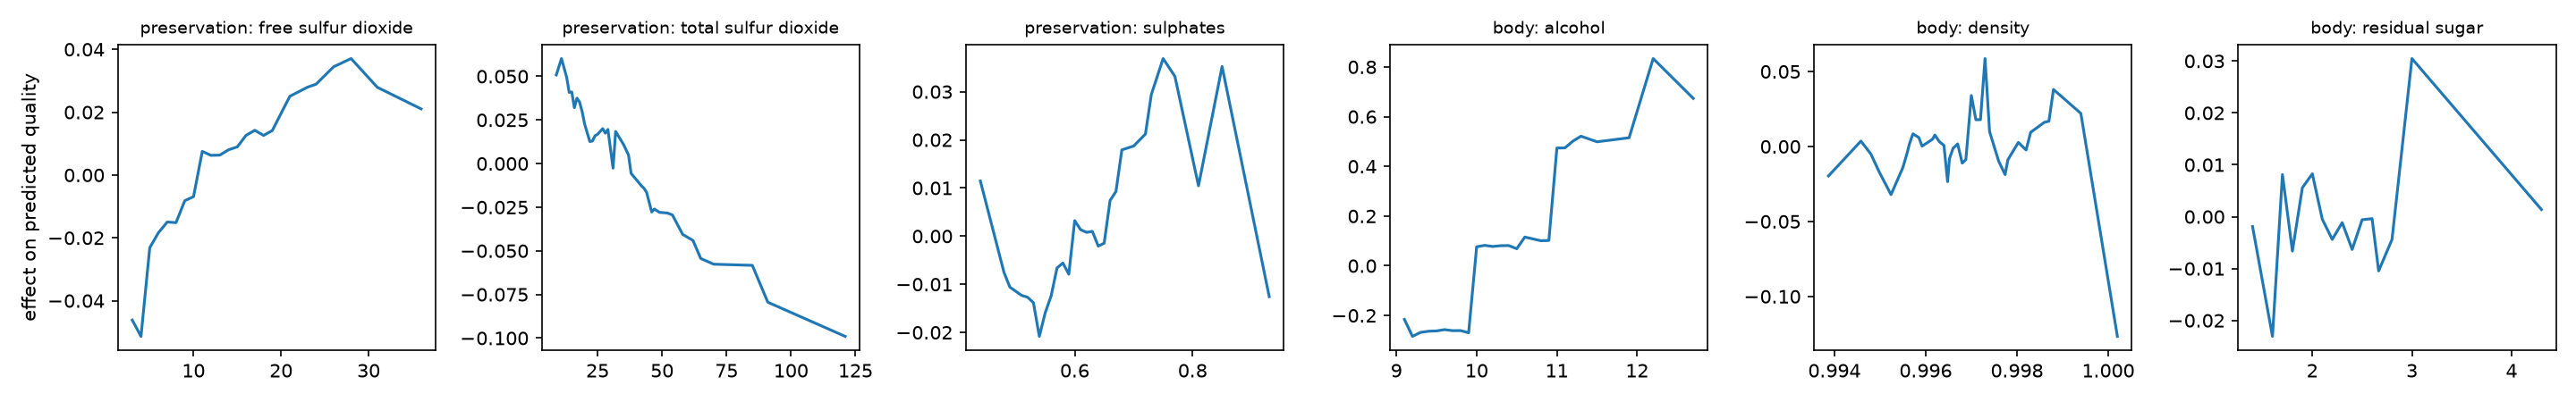
\includegraphics[width=\textwidth]{../figures/q4_cbm_pdp.png}
\caption{Top: learned concept weights and global importance (mean $|w_k(c_k-\bar c_k)|$). Bottom: partial dependence of the two active concepts on their features (effect on predicted quality, centred).}\label{fig:global}
\end{figure}

\sub{Global explanation.} The head learns $w=(0,\,0.27,\,0.97,\,0)$ for (acidity, preservation, body, salinity) with the full-data fit. The weights stay stable across seeds: body 0.96--0.97, preservation 0.27--0.29, acidity $\le$0.05, salinity 0. In practice the model uses \textbf{two concepts}: body accounts for 92\% and preservation for 8\% of the global importance. Inside them (Fig.~\ref{fig:global}), alcohol has a stepwise effect, with jumps near 10\% and 11\% vol. The predicted quality rises with free SO$_2$ and falls with total SO$_2$, and sulphates have a weaker, non-monotone effect. These directions agree with the univariate analysis in Q1. As a cross-check, grouped |SHAP| values of the unconstrained LightGBM rank the concepts the same way: body 76\%, preservation 11\%, acidity 8\%, salinity 4\%. The black box spreads a little importance over acidity and salinity, which the CBM ablation (Table~\ref{tab:cpt}) shows to be unnecessary.

\begin{figure}[h]\centering
\begin{subfigure}{0.6\textwidth}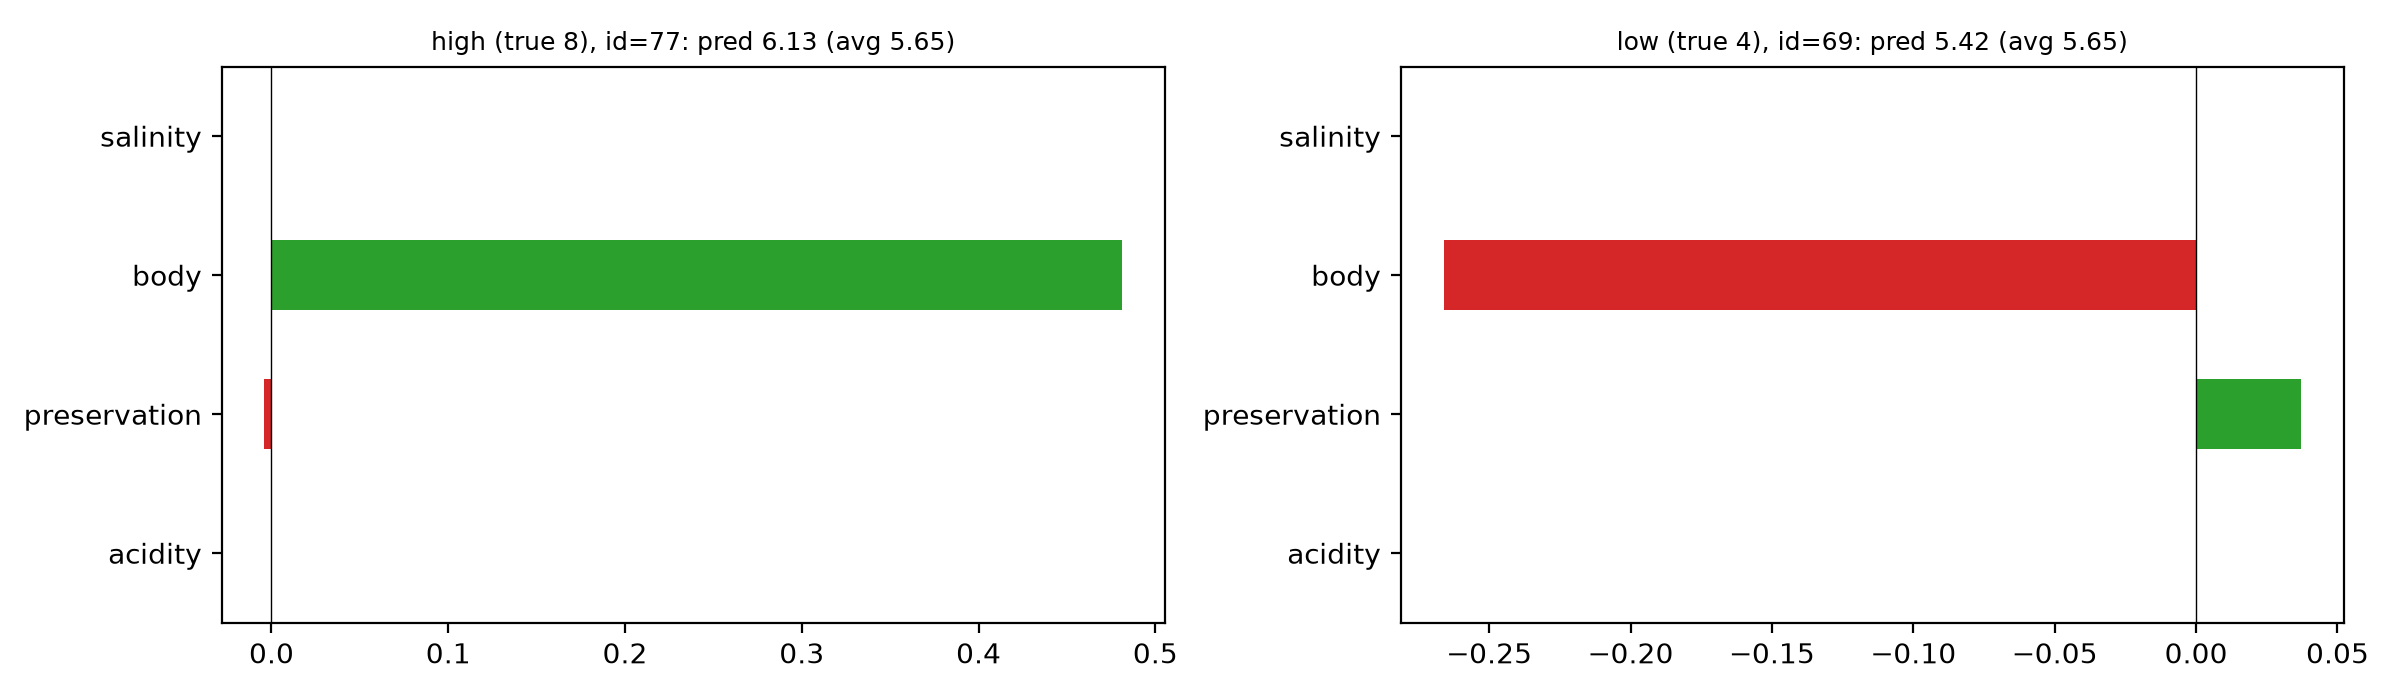
\includegraphics[width=\linewidth]{../figures/q4_case_study_cbm.png}\caption{CBM concept contributions $w_k(c_k(x)-\bar c_k)$.}\end{subfigure}\hfill
\begin{subfigure}{0.36\textwidth}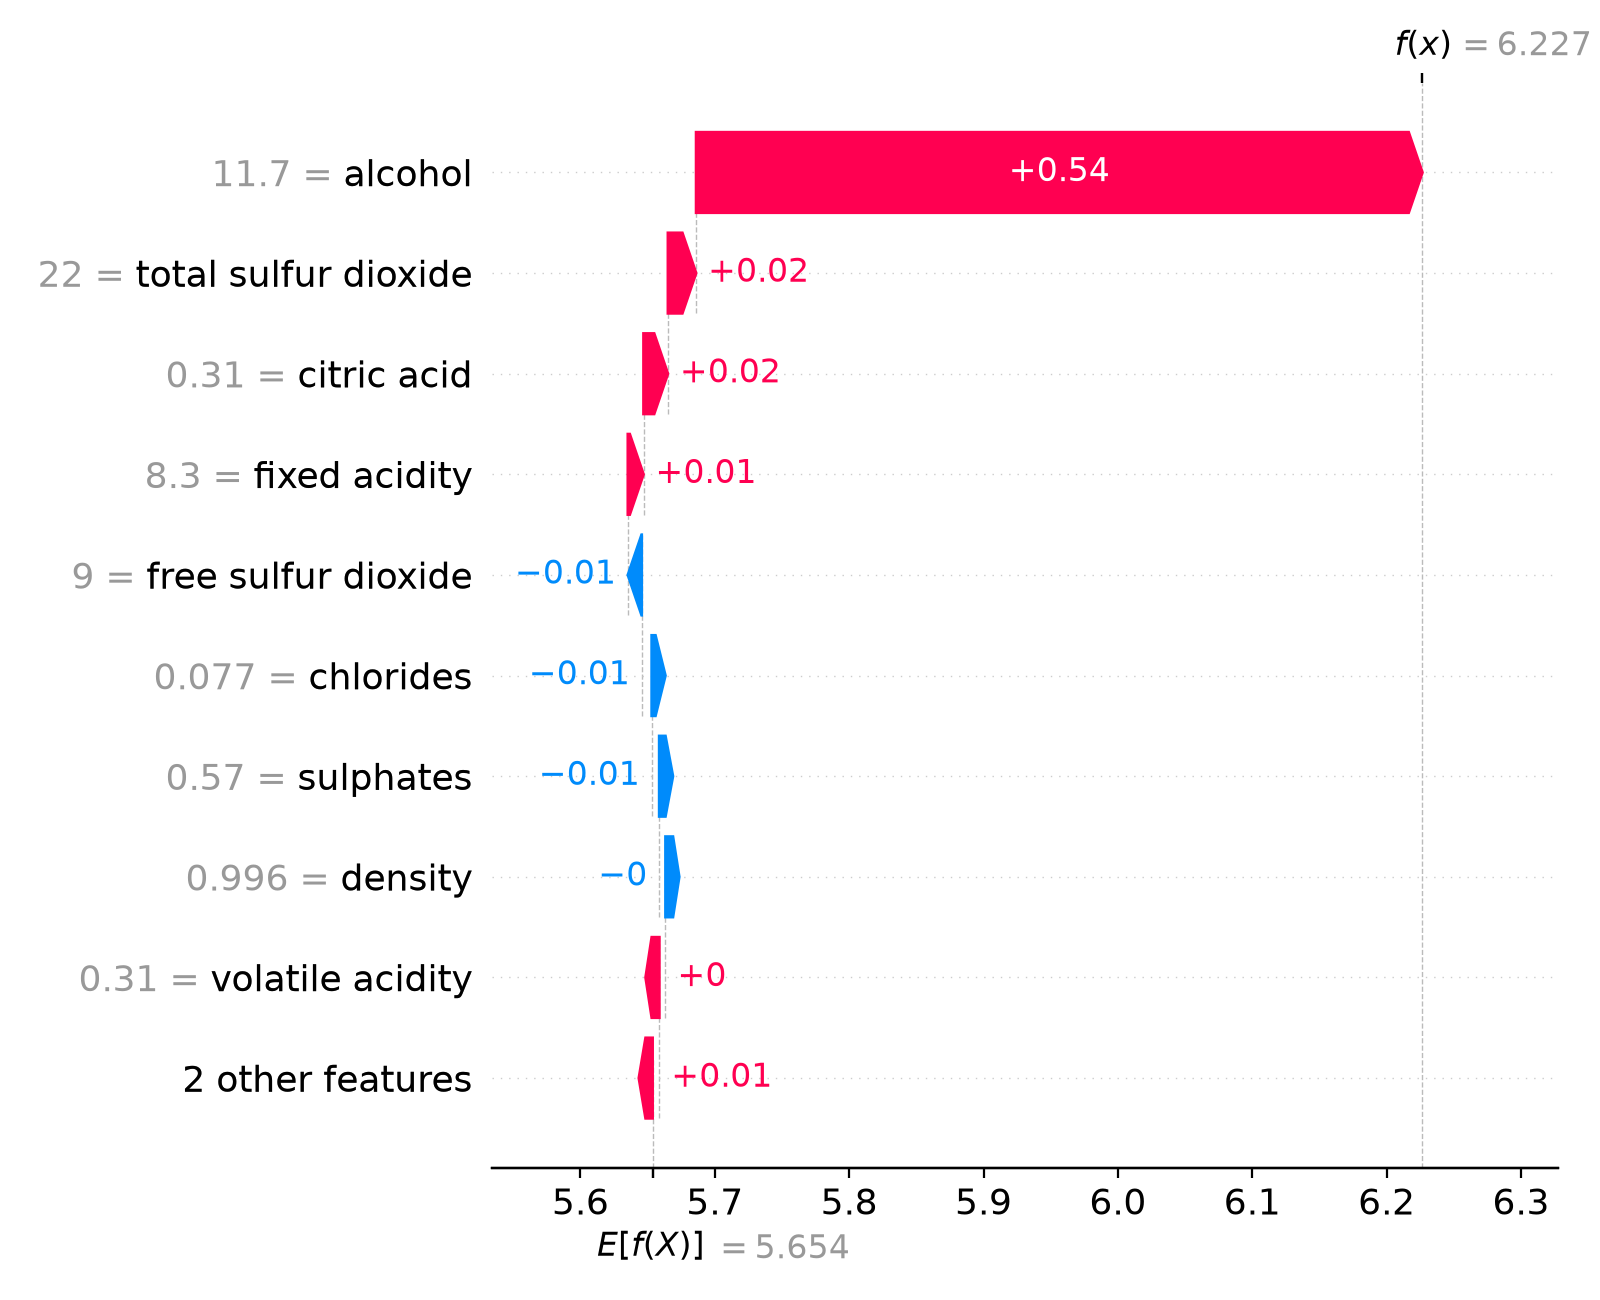
\includegraphics[width=\linewidth]{../figures/q4_case_study_shap.png}\caption{SHAP waterfall (LightGBM), wine 77.}\end{subfigure}
\caption{Case study of two training wines.}\label{fig:case}
\end{figure}

\sub{Case study} (Fig.~\ref{fig:case}). \textbf{Wine 77} (true quality 8; alcohol 11.7\%, total SO$_2$ 22, free SO$_2$ 9). The CBM predicts 6.13 against an average of 5.65, which the \texttt{v3\_cbm} thresholds map to class 7. Almost all of the +0.48 comes from \emph{body}, while \emph{preservation} is neutral (low free SO$_2$ cancels out low total SO$_2$). SHAP on LightGBM tells the same story: alcohol contributes +0.54 of the +0.57 gap ($5.65\rightarrow6.23$), and total SO$_2$ adds +0.02. Both explanations say the wine is rated highly \emph{because of its alcohol level}. The model under-predicts it by one class, as it does for most class-8 wines (only 21 of 204 are predicted as 8 out of fold), since 11.7\% alcohol is also common in class-6 and class-7 wines. \textbf{Wine 69} (true quality 4; alcohol 9.2\%, total SO$_2$ 53, sulphates 0.73). The CBM predicts 5.42 (class 5): \emph{body} pulls it down by $-0.27$, and \emph{preservation} pushes it up by $+0.04$ (free SO$_2$ 28 and sulphates 0.73 are favourable). The explanation also shows why the model errs: nothing among the features flags this wine as a 4, only a moderately low alcohol level, so the model stays near the dominant class 5. Errors like these are visible directly in the concept bars, without any external explainer.

\vspace{2pt}
{\small
\renewcommand{\refname}{\color{navy}\large References}
\begin{thebibliography}{9}\setlength{\itemsep}{0pt}\setlength{\parskip}{0pt}
\bibitem{cortez} P.~Cortez, A.~Cerdeira, F.~Almeida, T.~Matos, J.~Reis. Wine Quality. UCI Machine Learning Repository, 2009. doi:10.24432/C56S3T.
\bibitem{koh} P.~W.~Koh et al. Concept Bottleneck Models. ICML, 2020.
\bibitem{rudin} C.~Rudin. Stop explaining black box machine learning models for high stakes decisions and use interpretable models instead. Nature Machine Intelligence 1(5), 2019.
\bibitem{shap} S.~M.~Lundberg, S.-I.~Lee. A Unified Approach to Interpreting Model Predictions. NeurIPS, 2017.
\bibitem{ebm} H.~Nori, S.~Jenkins, P.~Koch, R.~Caruana. InterpretML: A Unified Framework for Machine Learning Interpretability. arXiv:1909.09223, 2019.
\end{thebibliography}}
\end{document}
